\chapter{进程与线程}

\section{进程与线程}

\subsection{进程的概念和特征}

    通常而言,在不同的认知角度上,对进程的定义是不同的,比较典型的定义为:

\begin{itemize}
    \item [1)] 进程是程序的一次执行过程
    \item [2)] 进程是一个程序及其数据在处理及上顺序执行时所发生的活动
    \item [3)] 进程是具有独立功能的程序在一个数据集合上运行的过程,是系统进行资源分配和调度的一个独立单位。
\end{itemize}

    当然的,在OS中,进程经过了抽象从而定义了一个重要的数据结构:进程控制块(Process Control Block,PCB)\footnote[1]{\emph{Linux中为task\_struct,定义在sche.h文件中}}。系统利用PCB来描述进程的基本情况和运行状态,进而控制和管理进程。\emph{相应地,由程序段、相关数据段和PCB三部分构成了进程实体(进程映像)。}

    注意:\emph{\color{red}PCB是进程存在的唯一标识}。

    \emph{进程映像可以被视为进程在内存中的静态表示,描述了进程的初始状态和资源分配情况。虽然进程映像在进程运行期间保持不变,但进程本身可能会发生动态的变化。}

    注意:\emph{\color{red}进程映像是静态的,进程则是动态的。}

    引入进程映像的概念后,又有了新的定义:\emph{进程是进程映像的运行过程,是系统进行资源分配和调度的一个独立单位。}

    进程是由多道程序的并发执行而引出的,其基本特征是对比单个程序的顺序执行提出的,也是对进程管理的基本要求:

\begin{itemize}
    \item [1)] 动态性。进程是程序的一次执行,{\color{red}动态性是进程最基本的特征}。
    \item [2)] 并发性。多个进程映像同存于内存中,能在一段时间内同时运行。{\color{red}并发性是进程的重要特征,也是OS的重要特征}。
    \item [3)] 独立性。进程映像是一个能独立运行、独立获得资源和独立接受调度的基本单位(此处暂时不考虑线程)。
    \item [4)] 异步性。由于进程的互相制约,使得进程各自独立、不可预知的向前推进。\emph{\color{red}异步性会导致执行的不可再现性,因此必须配置同步机制}。
\end{itemize}

\subsection{进程的状态与转换}

    进程在其生命周期内,会不断地发生状态变化。通常进程有五种状态,前三种是基本状态:

\begin{itemize}
    \item [1)] 运行态(Running)。进程正在CPU上运行。
    \item [2)] 就绪态(Runable)。进程获得了除处理机外的一切所需资源,\emph{通常处于就绪态的进程有多个,因此OS用就绪队列组织。}
    \item [3)] 阻塞态(Blocking/Waiting)。进程正在\emph{等待某一事件而暂停,通常处于阻塞态的进程有多个,因此OS用阻塞(等待)队列来组织,甚至可以根据阻塞原因设置多个阻塞队列。}
    \item [4)] 创建态(Creating)。进程正在被创建,未转到就绪态。
    \item [5)] 终止态(Exiting)。进程正在被释放或结束。
\end{itemize}

\begin{figure}[!htbp]
    \centering
    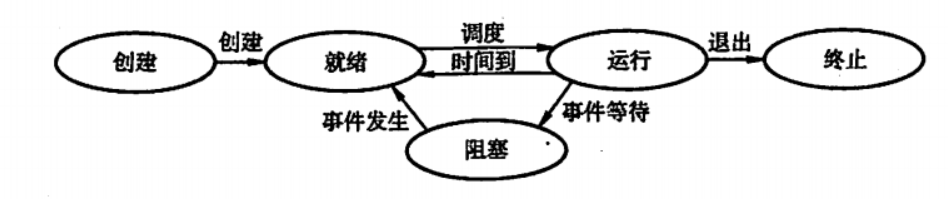
\includegraphics[width=0.8\textwidth]{image/chapter02/五种状态的转换.png}
    \caption{五种状态的转换}
\end{figure}

    值得注意的是:\emph{就绪态是指仅仅缺少处理机资源,也就是在就绪队列中还未到其处理的事件。而阻塞态是指,既缺乏处理机资源,又缺乏运行所需的必要资源(或事件发生)。}

    \emph{\color{red}一个进程从运行态变为阻塞态是主动的行为,从阻塞态变成就绪态是被动的行为。同时,就绪态不可能直接变为阻塞状态,因为变成阻塞必定是申请某种资源或事件发生,而这种情况之可能发生在运行时。}

\subsection{进程的组成}

    进程是一个独立的运行单位,也是OS进行资源分配和调度的基本单位。其由三个部分组成

\subsubsection{进程控制块}

    进程创建时,需要新建一个PCB常驻于内存中,PCB是进程存在的唯一标识,也是进程映射的一部分。

    \emph{在整个生命周期中,系统总是通过PCB对进程进行控制的,即系统唯有通过进程的PCB才能感知到该进程的存在。}

\begin{table*}[!htbp]
    \begin{center}
        \caption{PCB通常包含的内容}
        \begin{tabular}{c | c | c | c}
            \hline
            进程描述信息 & 进程控制和管理信息 & 资源分配清单 & 处理机相关信息 \\
            \hline
            进程标识符(PID) & 进程当前状态 & 代码段指针 & 通用寄存器值 \\
            \hline
            用户标识符(UID) & 进程优先级 & 数据段指针 & 地址寄存器值 \\
            \hline
            & 代码运行入口地址 & 堆栈指针 & 控制寄存器值 \\
            \hline
            & 程序外存地址 & 文件描述符 & 标志寄存器值 \\
            \hline
            & 进入内存时间 & 键盘 & 状态字 \\
            \hline
            & 处理机占用时间 & 鼠标 & \\
            \hline
            & 信号量使用 & & \\
            \hline
        \end{tabular}
    \end{center}
\end{table*}

\begin{itemize}
    \item [1)] 进程描述信息。\emph{\color{red}PID是进程的唯一标识符}。UID标识了进程所属的用户
    \item [2)] 进程控制和管理信息。
    \subitem 进程当前状态:描述进程的状态信息,作为调度的凭据
    \subitem 进程优先级:用于抢占机制
    \item [3)] 资源分配清单。用于说明内存地址空间或虚拟地址空间的状态,以及文件和I/O情况
    \item [4)] 处理机相关信息。用于保存进程的信息,当进程被切换时,必须将上下文信息保存在此处(线程就是为此的)。
\end{itemize}

    在OS中,为了满足各种情况,通常有:就绪队列,等待队列以及优先级队列,这三种队列都会保存在PCB中以供使用。

    特别的,一般而言还有另外一种组织方式:索引方式,将同一状态的进程组织在一张索引表内,然后通过索引表项指向PCB。

\subsubsection{程序段}

    程序段就是\emph{能够被进程调度程序调度到CPU执行的程序段代码。程序可能被多个进程共享。}

    代码段通常是只读的,意味着程序在运行时无法修改代码段中的指令。这是为了确保程序的逻辑和一致性。如果程序需要修改自身的指令,通常会使用特殊的技术,如自修改代码或动态代码生成。

    在计算机的内存中,代码段通常位于程序的虚拟地址空间的一个固定位置。操作系统负责将代码段加载到内存中,并为程序提供执行的环境和资源。

\subsubsection{数据段}

    一个进程的数据段,\emph{可以是进程对应的程序加工处理的原始数据,也可以是程序执行时产生的中间或最终结果。}

    进程的可变性,就主要体现在数据段中的变化。

\subsection{进程控制}

    进程控制的主要功能是对系统中的所有进程实施有效的控制,具有创建、删除、转换等原语。

\subsubsection{进程的创建}

    允许一个进程创建另一个进程。子进程可以继承父进程的所有资源。在OS中,系统调用的上层接口是fork(),而底层的原语接口是clone()。

    在OS中,终端用户登录系统、作业调度、系统提供服务、用户程序的应用请求等都会引起进程的创建:

\begin{itemize}
    \item [1)] 为新进程分配唯一的一个PID,并申请一个空白PCB。
    \item [2)] 为进程分配运行所需的各种资源。
    \item [3)] 初始化PCB,主要包括初始化标志信息、初始化CPU状态信息和初始化CPU控制信息,以及设置优先级
    \item [4)] 若进程就绪队列能够容纳,则并入就绪队列,等待被调度
\end{itemize}

\subsubsection{进程的终止}

    引起进程终止的事件主要有:正常结束;异常结束;外界干预这三种:

\begin{itemize}
    \item [1)] 根据被终止进程的标识符,检索出进程的PCB,从中读取进程状态
    \item [2)] 若被终止进程处于运行态,立即终止执行,并将处理机资源分配给其他任务
    \item [3)] 若该进程有子进程,则还应将子进程终止
    \item [4)] 将该进程的全部资源归还给父进程或OS
    \item [5)] 将该PCB从队列中移除
\end{itemize}

\subsubsection{进程的阻塞和唤醒}

    正在运行的任务,由于期待的事件尚未发生,进程便通过调用阻塞原语,使自身从运行态转变为阻塞状态。\emph{可见,阻塞态是一种进程的自身主动行为,因此只能处于在运行态的进程才可能转换为阻塞态}:

\begin{itemize}
    \item [1)] 找到将要被阻塞进程的标识号对应的PCB
    \item [2)] 若进程为运行态,则{\color{red}保护现场},将其转换为阻塞态,停止运行
    \item [3)] 将该PCB插入到对应事件的等待队列,将处理机资源调度给其他就绪任务
\end{itemize}

    当被阻塞进程所期待的事件发生时,由有关进程调用唤醒原语(Wakeup):

\begin{itemize}
    \item [1)] 在该事件的等待队列中找到响应的PCB
    \item [2)] 将其从等待队列中移除,并置为就绪态
    \item [3)] 把该PCB插入就绪队列,等待调度程序调度
\end{itemize}

    注意:\emph{阻塞和唤醒原语是一对作用相反的原语,因此需要成对使用。}

\subsubsection{进程的切换}

    进程的切换一般由于:当前进程时间片到;更高优先级任务到达;当前进程主动阻塞;当前进程终止等,这时就需要切换原语:

\begin{itemize}
    \item [1)] 将运行环境信息存入PCB
    \item [2)] PCB移入对应队列
    \item [3)] 选择另一个任务执行,更新PCB
    \item [4)] 根据PCB恢复新进程所需要的环境
\end{itemize}

    对于切换的原语,可以在内核中轻易的找到:

\begin{lstlisting}[language=C++]
#define switch_to(prev,next,last) \
asm volatile(SAVE_CONTEXT						    \
    "movq %%rsp,%P[threadrsp](%[prev])\n\t" /* save RSP */	  \
    "movq %P[threadrsp](%[next]),%%rsp\n\t" /* restore RSP */	  \
    "call __switch_to\n\t"					  \
    ".globl thread_return\n"					\
    "thread_return:\n\t"					    \
    "movq %%gs:%P[pda_pcurrent],%%rsi\n\t"			  \
    "movq %P[thread_info](%%rsi),%%r8\n\t"			  \
    "btr  %[tif_fork],%P[ti_flags](%%r8)\n\t"			  \
    "movq %%rax,%%rdi\n\t" 					  \
    "jc   ret_from_fork\n\t"					  \
    RESTORE_CONTEXT						    \
    : "=a" (last)					  	  \
    : [next] "S" (next), [prev] "D" (prev),			  \
    [threadrsp] "i" (offsetof(struct task_struct, thread.rsp)), \
    [ti_flags] "i" (offsetof(struct thread_info, flags)),\
    [tif_fork] "i" (TIF_FORK),			  \
    [thread_info] "i" (offsetof(struct task_struct, thread_info)), \
    [pda_pcurrent] "i" (offsetof(struct x8664_pda, pcurrent))   \
    : "memory", "cc" __EXTRA_CLOBBER)

struct task_struct *
__switch_to(struct task_struct *prev_p, struct task_struct *next_p)
\end{lstlisting}

\subsection{进程的通信}

    进程通信是指进程间的信息交换。PV操作是低级通信方式\footnote[1]{\emph{PV操作是一种用于进程同步的经典算法,用于解决进程之间的互斥和同步问题。PV操作通常与信号量(Semaphore)相关联。当进程需要访问共享资源时,执行P(wait)操作;当进程结束访问时,需要执行V(signal)操作。}},高级通信方式是指\emph{以较高的效率传输大量数据的通信方式}。

\subsubsection{共享存储}

    \emph{进程空间一般都是独立的,进程运行期间不能访问其他进程。}这是共享存储的前提条件,在通信的进程之间存在一块可以直接访问的共享空间,通过对该空间进行读写操作,实现进程间的消息互换。

\begin{figure}[!htbp]
    \centering
    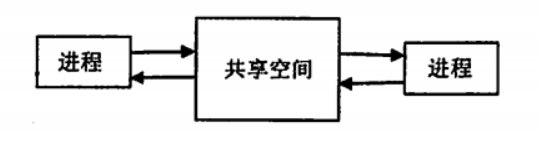
\includegraphics[width=0.6\textwidth]{image/chapter02/共享空间.png}
    \caption{共享存储}
\end{figure}

    为了实现共享存储,一般OS会提供上层接口以供使用。例如Linux中,提供了shm\_*等操作实现申请、撤销共享空间等操作,然后通过mmap将共享空间映射到进程自身的空间中。

    此处给出简单的示例:

\begin{lstlisting}[language=C++]
#include <stdio.h>
#include <stdlib.h>
#include <sys/mman.h>
#include <sys/stat.h>
#include <fcntl.h>
#include <unistd.h>
#include <sys/types.h>

int main() {
    const char* shm_name = "/my_shared_memory";
    int shm_fd = shm_open(shm_name, O_RDWR | O_CREAT, 0666);
    if (shm_fd == -1) {
        perror("shm_open");
        exit(1);
    }

    off_t size = 4096; // 共享内存的大小
    if (ftruncate(shm_fd, size) == -1) {
        perror("ftruncate");
        exit(1);
    }

    void* addr = mmap(NULL, size, PROT_READ | PROT_WRITE, MAP_SHARED, shm_fd, 0);
    if (addr == MAP_FAILED) {
        perror("mmap");
        exit(1);
    }

    // 现在可以通过addr指针来访问共享内存中的数据

    // 访问完成后,记得使用munmap函数解除映射
    if (munmap(addr, size) == -1) {
        perror("munmap");
        exit(1);
    }

    // 关闭共享内存文件描述符
    if (close(shm_fd) == -1) {
        perror("close");
        exit(1);
    }

    // 删除共享内存对象
    if (shm_unlink(shm_name) == -1) {
        perror("shm_unlink");
        exit(1);
    }

    return 0;
}
\end{lstlisting}

    对于共享存储而言,拥有两种方式:低级的共享是通过语言特性,例如全局的数据结构的共享,但是这样效率低、局限大;高级的共享就是通过这样实现一块存储区,速度快,局限小。

\subsubsection{消息传递}

    在消息传递系统中,进程间的数据交换以格式化的信息为单位。进程通过系统提供的发送/接收原语进行数据交换,\emph{这种方式隐藏了通信实现细节,使通信过程对用户透明,简化了通信程序的设计,是目前最广泛应用的机制。}

\begin{figure}[!htbp]
    \centering
    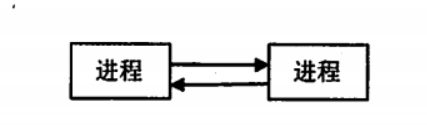
\includegraphics[width=0.4\textwidth]{image/chapter02/消息传递.png}
    \caption{消息传递}  
\end{figure}

\begin{itemize}
    \item [1)] 直接通信方式。发送进程直接把消息发送给接收进程,并将其挂在接收进程的消息缓冲队列上,接收进程从中获取消息。
    \item [2)] 间接通信方式。发送进程把消息发送到某个中间实体(类似于电子邮件的机制,是有一个邮件服务器的缓冲区),接收端从中间实体获取消息,该中间实体一般称为信箱。
\end{itemize}

\subsubsection{管道通信}

    \emph{在Linux中,管道是一种使用非常频繁的通信机制,本质上也是一种文件。}管道通信允许两个进程按生产-消费者模型进行通信,数据在管道中是FIFO的。管道的大小也是有规定的,一般为4KB(也就是说,是一个固定的缓冲区)。

    \emph{1. 管道只能采用半双工通信,某段时间内只能单向通信;但可以使用两个管道实现全双工通信。}

    \emph{2. 各进程需要互斥的读写管道。当管道写满时,写进程阻塞;当管道读空时,读进程堵塞。}

    \emph{3. 数据一旦被读取,一般情况下会消失。因此会出现争议:a). 一个管道允许多个写进程,一个读进程\footnote[1]{\emph{如果是答题,按照参考答案上的结果就是这样。如果从理解上来看,这种和后面一种的方式都是正确的。}}。b). 允许多个写进程,多个读进程,系统会让进程各自轮流读取\footnote[2]{\emph{Linux中的策略}}}。

    一个简单的示例,实现进程间互相通信:

\begin{lstlisting}[language=C++]
#include <stdio.h>
#include <stdlib.h>
#include <unistd.h>

int main() {
    int pipe1[2]; // 管道1,用于父进程向子进程发送数据
    int pipe2[2]; // 管道2,用于子进程向父进程发送数据

    if (pipe(pipe1) == -1 || pipe(pipe2) == -1) {
        perror("pipe");
        exit(1);
    }

    pid_t pid = fork();
    if (pid == -1) {
        perror("fork");
        exit(1);
    }

    if (pid == 0) {
        // 子进程
        close(pipe1[1]); // 关闭管道1的写端
        close(pipe2[0]); // 关闭管道2的读端

        char message[100];
        read(pipe1[0], message, sizeof(message)); // 从管道1读取数据
        printf("子进程收到消息:%s\n", message);

        const char* reply = "Hello, 父进程!";
        write(pipe2[1], reply, strlen(reply) + 1); // 向管道2写入数据

        close(pipe1[0]); // 关闭管道1的读端
        close(pipe2[1]); // 关闭管道2的写端
    } else {
        // 父进程
        close(pipe1[0]); // 关闭管道1的读端
        close(pipe2[1]); // 关闭管道2的写端

        const char* message = "Hello, 子进程!";
        write(pipe1[1], message, strlen(message) + 1); // 向管道1写入数据

        char reply[100];
        read(pipe2[0], reply, sizeof(reply)); // 从管道2读取数据
        printf("父进程收到消息:%s\n", reply);

        close(pipe1[1]); // 关闭管道1的写端
        close(pipe2[0]); // 关闭管道2的读端
    }

    return 0;
}
\end{lstlisting}

\subsection{线程和多线程模型}

\subsubsection{线程的基本概念}

    \emph{引入线程的目的是减少程序在并发执行时所付出的时空开销,提高OS的并发性能。}

    线程最为直接的理解就是“轻量级进程”,\emph{是一个基本的CPU执行单元,也是程序执行流的最小单元。}线程是进程的一个实体,\emph{{\color{red}是被OS独立调度和分派的基本单位}(引入线程后,进程就不再是调度的基本单位了),线程不拥有系统资源,但可以与同属进程的其他线程共享所拥有的全部资源。}

    那么,现在重新定义:\emph{进程是只作为除CPU外的系统资源的分配单元,线程作为处理机的分配单元。}

\subsubsection{线程与进程的比较}

\begin{itemize}
    \item [1)] 调度
    \subitem 引入线程后,\emph{线程是独立调度的基本单位},线程切换的代价远小于进程,同时,在同一进程中的不同线程切换,不需要切换进程。
    \item [2)] 并发性
    \subitem 不仅进程能够并发,线程也是能够并发的,准确来说,线程就是为此而生的
    \item [3)] 拥有资源
    \subitem \emph{进程是系统中拥有资源的基本单位,线程不拥有系统资源,但能够访问所属进程的资源(主要表现在,同一进程中的所有线程具有相同的地址空间)}
    \item [4)] 独立性
    \subitem \emph{每个进程都拥有独立的地址空间和资源,除了共享的全局变量;而同一进程的所属线程间,共享进程的地址空间和资源。}
    \item [5)] 系统开销
    \subitem 显然,线程的各种开销明显小于进程
    \item [6)] 支持多处理机系统
\end{itemize}

\subsubsection{线程的状态和转换}

    与进程类似,各线程间因为并发的原因也存在共享资源和相互合作的制约关系:

\begin{figure}[!htbp]
    \centering
    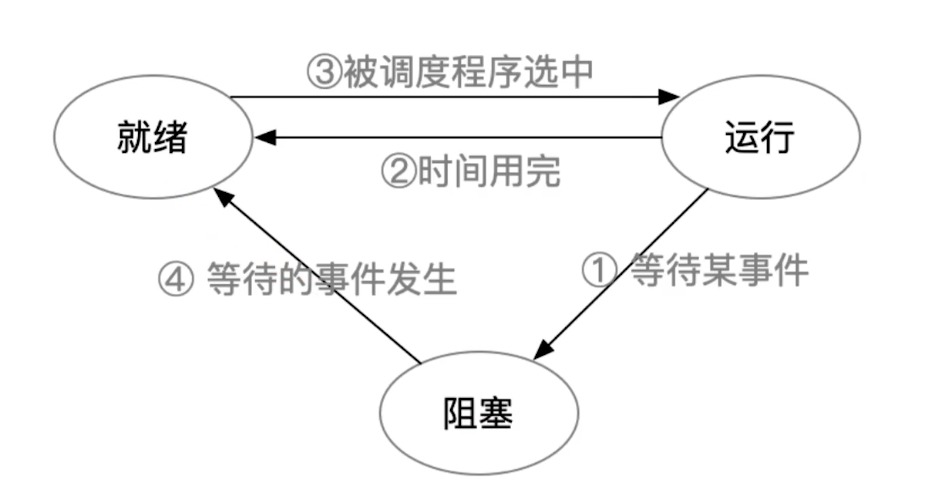
\includegraphics[width=0.6\textwidth]{image/chapter02/线程的状态与转换.png}
    \caption{线程的状态与转换}
\end{figure}

\subsubsection{线程的组织与控制}

    与进程类似,OS也为线程配置了一个线程控制块TCB,用于记录控制和管理线程的信息。

\begin{figure}[!htbp]
    \centering
    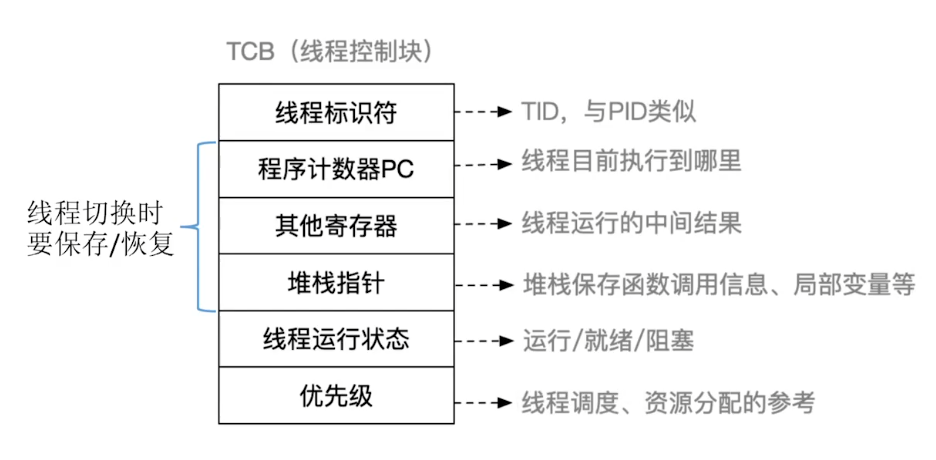
\includegraphics[width=0.6\textwidth]{image/chapter02/TCB.png}
    \caption{TCB}
\end{figure}

    同一进程中所有线程都完全共享进程的空间与资源,一个线程能够读写甚至删除另一个线程的堆栈。同时,线程的创建和终止也和进程类似,不过在删除时,必须考虑进程的因素,从而选择是否释放资源。

\subsubsection{线程的实现方式}

    线程的实现可以分为两类:用户级线程(User-Level Thread,ULT)和内核级线程(Kernel-Level Thread)

\paragraph{用户级线程}

    \emph{在用户级线程中,有关线程管理的所有工作都是由应用程序在用户态完成的,{\color{red}内核根本意识不到线程的存在}。}因此,对于设置了ULT的系统,其调度实际上还是以进程为单位的。

    这种方式的优点在于:

    \emph{1. 线程切换不需要进入到内核态,节省了切换的开销。}

    \emph{2. 调度算法是进程专用的,不同进程可根据自身需求,为自己的线程选择不同的调度算法。}

    \emph{3. 用户级线程的实现与OS无关,对线程管理的代码属于用户程序的一部分}

    而缺点在于:

    \emph{1. 系统调用的阻塞不仅会导致该进程被阻塞,且进程内的所有线程都会被阻塞}

    \emph{2. 严重降低了处理效率,不能发挥多处理机的优势}

\paragraph{内核级线程}

    内核级线程是由内核支持的,线程管理的工作在内核空间中实现。因此内核为每个线程设置了TCB,\emph{\color{red}内核能够对内核级线程进行感知。}

    这种方式的优点在于:

    \emph{1. 发挥了多处理机的优势,能够同时调度同一进程中的多个线程}

    \emph{2. 如果进程中的一个线程阻塞,那么可以对另外一个线程进行调度}

    \emph{3. 内核支持线程具有小的数据结构和堆栈,切换较快,开销较小}

    \emph{4. 内核本身也提供多线程技术,提高系统的执行效率}

    而缺点在于:

    \emph{同一进程中的线程切换,需要转换到内核态,系统开销较大。}

\paragraph{ULT \& KLT}

    ULT和KLT的组合能够使得结合各自的优点并克服各自的不足。支持多个内核级线程的建立、调度和管理,同时允许用户级线程的使用,能够使得线程阻塞但不会导致其他线程阻塞。

\begin{figure}[!htbp]
    \centering
    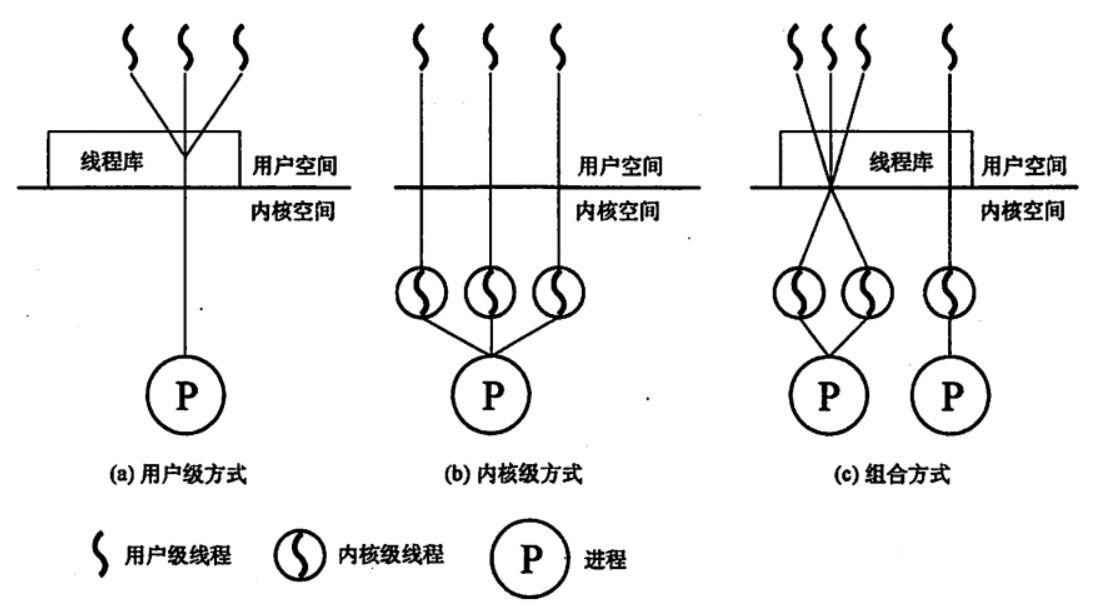
\includegraphics[width=0.8\textwidth]{image/chapter02/用户级线程和内核级线程.png}
    \caption{用户级线程和内核级线程}
\end{figure}

\subsubsection{多线程模型}

    基于有些系统同时支持用户线程和内核线程,因此就会产生不同的多线程模型:

\paragraph{多对一模型}

    将多个用户级线程映射到一个内核级线程(一般来说,多对一就是特指一个内核级线程),这些用户级线程通常属于一个进程。

    优点:线程管理在用户空间进行,效率较高

    缺点:一个线程发生阻塞,那么整个进程都会阻塞;且任何时刻只能由一个线程访问内核

\paragraph{一对一模型}

    每个用户级线程映射到一个内核级线程

    优点:当一个线程被阻塞后,允许调度另一个线程,并发能力较强

    缺点:每创建一个用户线程,都需要一个内核线程,开销过大

\paragraph{多对多模型}

    将n个用户级线程映射到m个内核级线程,要求$n \geq m$

    特点:既克服了多对一模型并发度不高的缺点,又克服了一对一模型开销过大的问题。

\begin{figure}[!htbp]
    \centering
    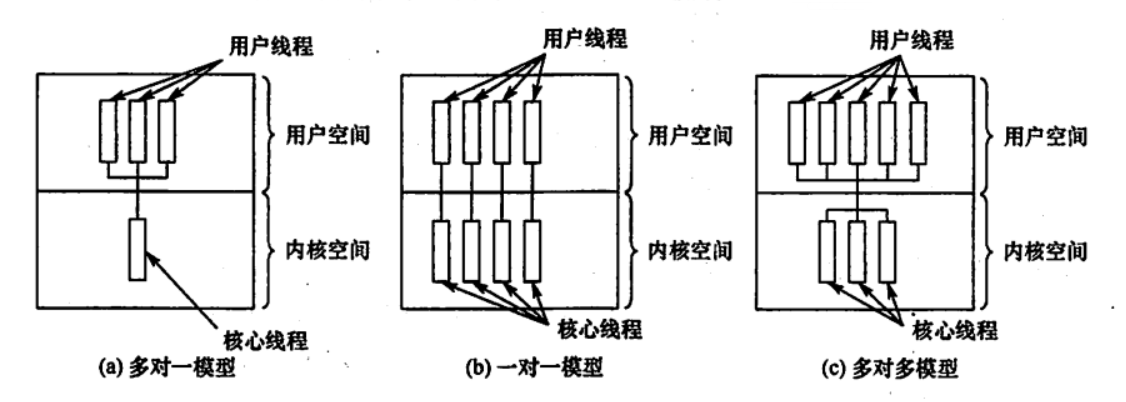
\includegraphics[width=0.8\textwidth]{image/chapter02/多线程模型.png}
    \caption{多线程模型}
\end{figure}

\section{处理机调度}

\subsection{调度的概念}

\subsubsection{调度的基本概念}

    \emph{处理机调度是对处理机进行分配,即从就绪队列中按照一定的算法选择一个进程并将处理机分配给它允许,以实现进程的并发执行}

\subsubsection{调度的层次}

    一个作业(也就是一个程序)从提交到完成,往往经历以下三级调度:

\begin{itemize}
    \item [1)] 高级调度(作业调度)
    \subitem 按照一定的原则从\emph{外存中处于后备队列中的作业中}挑选一个(或多个),给他们分配内存、输入/输出等必要资源,\emph{\color{red}并建立对应的PCB}。
    \subitem \emph{作业调度是内存与辅存之间的调度,\color{red}每个作业只调入一次、调出一次。}
    \item [2)] 中级调度(内存调度)
    \subitem 中级调度的目的是为了\emph{提高内存利用率和系统吞吐量。}可以将暂时不能运行的进程调至外存等待,此时进程的状态为\emph{\color{red}挂起态}\footnote[1]{\emph{挂起态可以分为就绪挂起和阻塞挂起,这就是七状态模型。}}
    \subitem 当其具备运行条件且内存有足够的空闲时,修改其状态为就绪态,挂在就绪队列中等待。\emph{中级调度实际上是存储器管理中的对换功能(swap)}。
    \item [3)] 低级调度(进程调度)
    \subitem 按照某种算法从就绪队列中选取一个进程,将处理机分配给它。\emph{调度算法是最基本的一种调度,在各种OS中必须配置该调度。}
\end{itemize}

\begin{figure}[!htbp]
    \centering
    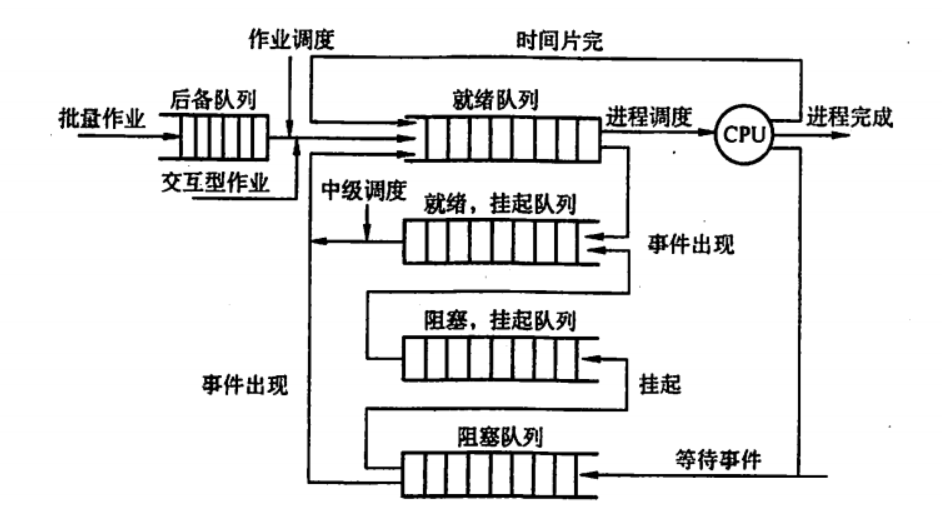
\includegraphics[width=0.8\textwidth]{image/chapter02/处理机三级调度.png}
    \caption{处理机的三级调度}
\end{figure}

\subsubsection{三级调度的联系}

    作业调度从外存中的后备队列选择一批作业进入内存,且创建对应的PCB,然后送入就绪队列中,进程调度从就绪队列选择一个进程,将其状态改为运行态,并分配处理及资源。中级调度为了提高内存利用率。

\begin{itemize}
    \item [1)] 作业调度为进程活动做准备,进程调度使进程正常活动
    \item [2)] 作业调度次数少,中级调度略多,进程调度频率最高
    \item [3)] 进程调度是最基本的,不可或缺
\end{itemize}

\subsection{调度的目标}

\begin{itemize}
    \item [1)] CPU利用率
    \subitem CPU是OS中最重要和昂贵的资源之一,因此应该尽可能使CPU保持“忙”状态:
    \subitem $$CPU_{Utilization} = \frac{CPU_{efficient}}{CPU_{efficient} + CPU_{free}}$$
    \item [2)] 系统吞吐量
    \subitem 表示单位时间内CPU完成作业的数量。
    \item [3)] 周转时间
    \subitem 指从\emph{作业提交}到\emph{作业完成}所经历的时间,是\emph{作业等待、在就绪队列中排队、运行和输入/输出操作所花费时间的总和}:
    \subitem $$Turnaround = Work_{done} - Work_{submit}$$
    \subitem 平均周转时间是指多个作业周转时间的平均值
    \subitem $$Avr_{Turnaround} = \frac{Turnaround_1 + Turnaround_2 + \dots + Turnaround_n}{n}$$
    \subitem 带权周转时间是指作业周转时间与作业实际运行时间的比值
    \subitem $$P_{Turnaround} = \frac{Turnaround}{Real_{time}}$$
    \subitem 平均带权周转时间
    \subitem $$Avr_{PT} = \frac{P_{Turnaround}1 + \dots + P_{Turnaround}n}{n}$$
    \item [4)] 等待时间
    \subitem 指进程处于等待处理机的时间之和,等待时间越长,用户满意度越低。\emph{\color{red}处理机调度算法实际上不影响作业执行或输入/输出的时间,只影响作业在就绪队列中等待所花的时间}。\footnote[1]{\emph{值得注意的是,\color{red}等待IO并不算在等待时间,因为此时是正在被服务的。}}
    \item [5)] 响应时间
    \subitem 指从用户提交到系统首次执行或输入/输出操作的时间。\emph{在交互式系统中,周转时间往往不是最好的评价准则,一般采用响应时间作为衡量调度算法的重要准则之一。}
\end{itemize}

\subsection{调度的实现}

\subsubsection{调度程序(调度器)}    

    用于调度和分派CPU的组件称为调度程序,通常由三部分组成:

\begin{itemize}
    \item [1)] 排队器。将系统中的所有就绪进程按照一定的策略排成一个或多个队列。
    \item [2)] 分派器。依据调度程序中所选的进程,将其从就绪队列中取出,将CPU分配给新进程。
    \item [3)] 上下文切换器。在调度的时候,会发生切换,因此需要保存各自进程中的上下文数据。
\end{itemize}

\begin{figure}[!htbp]
    \centering
    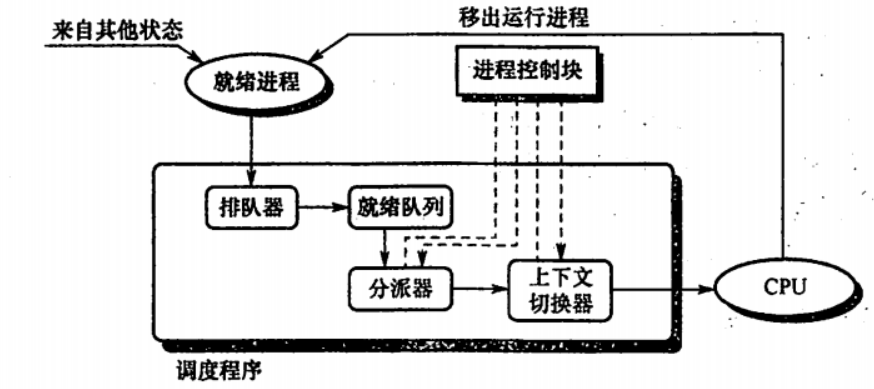
\includegraphics[width=0.6\textwidth]{image/chapter02/调度程序的结构.png}
    \caption{调度程序的结构}
\end{figure}

\subsubsection{闲逛进程}

    在进程切换时,如果系统中没有就绪进程,就会调度闲逛进程(idle)运行。\emph{闲逛进程的优先级最低,只有没有任何进程时,才会运行闲逛进程。}

    \emph{\color{red}闲逛进程不需要CPU之外的资源,其不会被堵塞。}

\subsection{调度算法}

\subsubsection{先来先服务(FCFS)调度算法}

    FCFS算法是一种最简单的调度算法,即可用于作业调度,也可用于进程调度。\emph{其主要从“公平”的角度考虑,按照作业/进程到达的先后顺序进行服务。}

    同时,FCFS算法是非抢占式算法,其优点\emph{在于简单、公平};缺点在于\emph{对短作业及其不友好。}\emph{\color{red}不会导致饥饿的情况}。

\begin{table*}[!htbp]
    \begin{center}
        \caption{FCFS调度算法的性能}
        \begin{tabular}{c | c | c | c | c | c | c | c }
            \hline
            作业号 & 提交时间 & 运行时间 & 开始时间 & 等待时间 & 完成时间 & 周转时间 & 带权周转时间 \\
            \hline
            1 & 8 & 2 & 8 & 0 & 10 & 2 & 1 \\
            \hline
            2 & 8.4 & 1 & 10 & 1.6 & 11 & 2.6 & 2.6 \\
            \hline
            3 & 8.8 & 0.5 & 11 & 2.5 & 11.5 & 2.7 & 5.4 \\
            \hline
            4 & 8.9 & 0.2 & 11.5 & 2.5 & 11.7 & 2.7 & 13.5 \\
            \hline
        \end{tabular}
    \end{center}
\end{table*}

\subsubsection{短作业优先(SJF)调度算法}

    短作业优先算法是指对短作业优先调度的算法,是非抢占式的,一般而言,\emph{非抢占式的短作业调度算法是指短进程优先调度算法(SPF),不过通常不会特别区分。}

    SJF算法的优点在于,能够使得平均等待/周转/带权周转时间均比FCFS要好,但是\emph{SJF对长作业不友好,容易导致长作业发生饥饿甚至饿死的情况。}

    同时注意:\emph{SJF算法并非是平均等待时间、平均周转时间最少的算法(\color{red}除非特别指明是SRNT算法)}。

\subsubsection{最短剩余时间优先(SRTN)调度算法}

    SRTN算法是基于SJF的调度算法,不过SRTN是{\color{red}可抢占的},\emph{每当加入一个新的进程,就绪队列就需要判断是否发生调度,如果新的进程运行时间比当前进程的剩余运行时间短,那么就发生调度。}

    因此,\emph{SRTN算法是平均等待时间、平均周转时间最少的算法(相较于这几种算法)。}

    同时,可以给出另一种定义:\emph{\color{red}在所有进程几乎同时到达时,采用SJF算法的平均等待时间、平均周转时间最少。}

    并且:\emph{由于SJF算法的作业的时间长短由用户提供的估计执行时间决定,因此可能导致用户无意间缩短其运行时间,因此\color{red}SJF不一定能够实现真正意义上的短作业优先}。

\subsubsection{高响应比优先(HRRN)调度算法}

    HRRN算法主要用于作业调度,是对FCFS和SJF算法的一种综合平衡,同时考虑了作业的等待时间和运行时间。

    \emph{在每次调度时,先计算每个作业的响应比,选择响应比高的作业进行调度:}

$$
    Response_{R_p} = \frac{Time_{wait} + Time_{Service}}{Time_{Service}}
$$

    是一种非抢占式调度算法,\emph{1. 作业的等待时间相同时,要求服务时间越短,响应比越高;2. 要求服务时间相同时,响应比取决于等待时间;3. 对于长作业,响应比可以随等待时间增加而提高,因此能够克服饥饿现象。}

    \emph{上面的几种调度算法,主要用于早期的批处理OS,因此几乎都不关心响应时间,而更在乎整体性能。}

\subsubsection{时间片轮转(RR)调度算法}

    时间片轮转调度算法主要用于分时系统,\emph{更注重响应时间,忽略周转时间。轮流让就绪队列中的进程依次执行一个时间片。}

    注意:\emph{\color{red}如果一个时间片用完时,刚好另一个任务被提交上来,那么新加入的任务优先进入队列。}

    时间片轮转的好处是显而易见的,但是,\emph{如果时间片设置过大,那么就会退化为FCFS调度算法,并且增大进程响应时间;如果时间片过小,又会导致进程切换过于频繁,使得资源开销过大}。

    一般来说,\emph{\color{red}设计时间片时要让切换进程的开销占比不超过1\%。}

\subsubsection{优先级调度算法}

    优先级调度算法既可用于作业调度,又可用于进程调度。\emph{主要描述一个作业的紧急程度。}

    \emph{优先级算法每次从后备队列中选取优先级最高的任务进行调度,可以分为抢占式和非抢占式:}

\begin{itemize}
    \item [1)] 非抢占式优先级调度。每次选择已到达任务中优先级最高的任务进行调度
    \item [2)] 抢占式优先级调度。根据每次到达任务中优先级最高的任务进行调度
\end{itemize}

    对于优先级来说,进程可以设置两种不同的优先级:

\begin{itemize}
    \item [1)] 静态优先级。创建进程时就已经确定,且保持运行期间不会发生改变。
    \item [2)] 动态优先级。根据进程情况的变化动态调整优先级。
    \begin{itemize}
        \item [a)] 系统进程 > 用户进程。系统的优先级理应高于用户
        \item [b)] 交互型进程 > 非交互型进程。需要交互的进程需要更快的响应速度。
        \item [c)] I/O型进程 > 计算型进程。I/O设备一般比CPU运行的更慢,能够更快进行I/O设备的调度就能够使得等待时间和响应更快,提升OS的整体效率
    \end{itemize}
\end{itemize}

\subsubsection{多级队列调度算法}

    在多处理机中,上述都是单一的调度策略,多级队列设置多个就绪队列,将不同类型或性质的进程固定分配到不同的就绪队列。

\subsubsection{多级反馈队列调度算法}

    多级反馈队列调度算法是时间片轮转调度算法和优先级算法的综合发展,通过\emph{\color{red}动态调整进程优先级和时间片大小},能够兼顾多方面的系统目标。

    \emph{各级队列优先级从高到低、时间片从小到大;新进程进入按照FCFS算法进入最高优先级队列,{\color{red}若在一个时间片内无法结束,那么降级到第二级优先级}。只有当上级队列为空时,才能够调度下一级队列中的任务。}

\begin{figure}[!htbp]
    \centering
    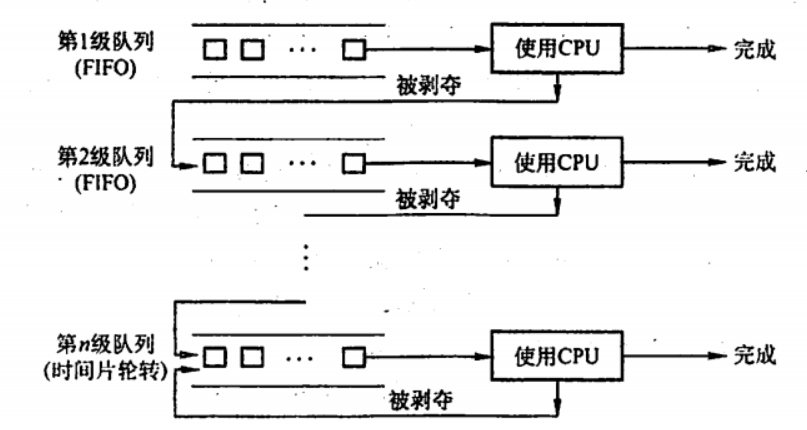
\includegraphics[width=0.6\textwidth]{image/chapter02/多级反馈队列调度算法.png}
    \caption{多级反馈队列调度算法}
\end{figure}

\subsection{进程切换}

    狭义的进程调度指的是\emph{将一个任务从就绪队列中调度上CPU的动作};而进程切换通常指的是\emph{一个任务让出处理机,另一个任务占用,会涉及到上下文切换。}对于广义的进程调度,则是都包含。

\subsubsection{上下文切换}

    从CPU上切换一个任务需要保存当前任务状态,并恢复另一个任务的状态,同时需要恢复其环境,这个过程叫做上下文切换。\emph{上下文指的是某一时刻CPU寄存器和程序计数器中的内容。}

\begin{itemize}
    \item [1)] 挂起一个进程,保存CPU上下文
    \item [2)] 更新PCB信息
    \item [3)] 把进程的PCB移入相应的队列
    \item [4)] 选择另一个进程执行,更新其PCB
    \item [5)] 跳转到新进程PCB中的程序计数器所指向的位置执行
    \item [6)] 恢复处理机上下文
\end{itemize}

\subsubsection{上下文切换与模式切换}

    通常而言,模式切换指的是\emph{用户态与内核态之间的状态切换,其不会改变当前进程。}上下文切换\emph{\color{red}只会发生在内核态,是多任务OS中的一个必需的属性。}

\section{同步与互斥}

\subsection{同步与互斥的基本概念}

\subsubsection{临界资源}

    \emph{在OS中,多个进程可以共享各种资源,但其中许多资源一次只能为一个进程使用,因此\color{red}将一次仅能一个进程使用的资源称为临界资源}。

    对临界资源的访问必须互斥的进行,每个进程中,\emph{访问临界资源的那段代码称为临界区}:

\begin{itemize}
    \item [1)] 进入区。检查进程是否能够使用临界资源,且阻止其他进程同时进入临界区。
    \item [2)] 临界区。进程中访问临界资源的代码段
    \item [3)] 退出区。修改临界标志
    \item [4)] 剩余区。代码中其余部分
\end{itemize}

\subsubsection{同步}

    同步可以称为\emph{直接制约关系,指为完成某种任务而建立的两个或多个进程,因为需要在某些位置上协调工作次序而等待、传递信息所产生的制约关系。}

\subsubsection{互斥}

    互斥可以称为\emph{间接制约关系,当一个进程进入临界区后,另一个进程必须等待其完成才能访问。}

    为禁止两个进程同时进入临界区,同步机制应遵循:

\begin{itemize}
    \item [1)] 空闲让进。临界区空闲时,可以允许一个请求进入临界区的进程立即进入
    \item [2)] 忙则等待。当已有进程进入临界区时,其他试图进入临界区的进程必须等待
    \item [3)] 有限等待。对请求访问的进程,应保证能在有限时间内进入临界区
    \item [4)] 让权等待。当进程不能进入临界区时,应立即释放处理器,防止进程忙等待
\end{itemize}

\subsection{实现临界区互斥的基本方法}

\subsubsection{软件实现方法}

\paragraph{单标志法}

    \emph{通过设置一个公用整型变量,用于指示被允许进入临界区的进程编号。}该算法良好的保证了一次只允许一个进程进入,\emph{\color{red}但两个进程必须交替进入,若某个进程不再进入,另一个进程则也无法进入:违背空闲让进原则}。

\begin{lstlisting}[language=C++]
P0:                         P1:
    while (turn != 0) ;         while (turn != 1) ;
    critical section ;          critical section ;
    turn = 1 ;                  turn = 0 ;
    remainder section ;         remainder section ;
\end{lstlisting}

\paragraph{双标志法先检查}

    \emph{通过在进程访问临界区资源之前,先检查临界区资源是否被访问,若正在被访问,则等待。}该算法避免了交替进入,\emph{但是由于两个进程并发可能“同时”进入临界区导致违背忙则等待原则}。

\begin{lstlisting}[language=C++]
P0:                             P1:
    while (flag[0]) ;               while (flag[1]) ;
    flag[1] = true ;                flag[0] = true ;
    critical section ;              critical section ;
    flag[0] = false ;               flag[1] = false ;
    remainder section ;             remainder section ;
\end{lstlisting}

\paragraph{双标志法后检查}

    \emph{为了防止同时进入临界区,可以先标识自身,然后检查对方的意愿。}避免了同时进入临界区,\emph{但导致了更严重的问题,二者都无法进入临界区使得\color{red}饥饿现象的出现}。

\begin{lstlisting}[language=C++]
P0:                             P1:
    flag[0] = true ;                flag[1] = true ;
    while (flag[1]) ;               while (flag[0]) ;
    critical section ;              critical section ;
    flag[0] = false ;               flag[1] = false ;
    remainder section ;             remainder section ;   
\end{lstlisting}

\paragraph{Peterson's Algorithm} 

    \emph{为了防止进程进入临界区无限期等待,设置一个类似于单标志法的共有变量,主体是双标志法和单标志法的综合。}

\begin{lstlisting}[language=C++]
P0:                             P1:
    flag[0] = true ;                flag[1] = true ;
    turn = 1;                       turn = 0;
    while (flag[1] && turn == 1) ;  while (flag[0] && turn == 0) ;
    critical section ;              critical section ;
    flag[0] = false ;               flag[1] = false ;
    remainder section ;             remainder section ;     
\end{lstlisting}

\subsubsection{硬件实现方法}

    \emph{计算机硬件提供了特殊的指令,允许对一个字中的内容进行检测和修整,或进行交换等,通过硬件支持实现临界段问题的方法称为低级方法,或元方法。}

\paragraph{中断屏蔽方法}

    \emph{一个进程正在执行临界区代码时,防止其他进程进入的最简方法是关中断。}但是,这种方法限制了处理机交替执行程序的能力,且中断指令是内核态的特权指令。

\paragraph{硬件指令方法}

\subparagraph{TestAndSet指令}

    又称TS或TSL指令。该指令是原子操作,即执行该代码时不允许被中断。其功能是读出指定标志后把该标志设置为真:

\begin{lstlisting}[language=C++]
bool TestAndSet (bool* lock) {
    bool old = *lock;
    *lock = true;
    return old;
}

while (TestAndSet(&lock)) ;
...
lock = false;
...
\end{lstlisting}

\subparagraph{Swap指令}

    又称Exchange或XCHG指令。

\begin{lstlisting}[language=C++]
void Swap (bool* a, bool* b) {
    bool temp = *a;
    *a = *b;
    *b = temp;
}
\end{lstlisting}

    值得注意的是,上述的C代码仅仅是对其功能的描述,真实的设计是在硬件上直接完成的。

    \emph{硬件方法的优点在于:适用于任意数目的进程,简单、容易检验其正确性,支持多个临界区。}

    \emph{其缺点在于:不能实现让权等待原则,可能导致饥饿现象。}

\subsection{互斥锁}

    \emph{解决临界区最简单的工具就是互斥锁(mutex lock)。}值得注意的是,互斥锁的申请和释放都必须是原子操作。\emph{互斥锁的主要缺点是忙等待,因为在进入临界区判断时,会一直自旋。}

    \emph{需要连续循环忙等的互斥锁,可以叫做自旋锁(spin lock)。}

\begin{lstlisting}[language=C++]
acquire() {
    while (!available) ;
    available = false;
}

release() {
    available = true;
}
\end{lstlisting}

\subsection{信号量}

    \emph{信号量机制时一种功能较强的机制,用于解决互斥同步问题,由OS提供的一对原语:wait和signal操作。}

    \emph{一般来说,这对原语也被称为PV操作,因此P(S)和V(S)分别代表了wait(S)和signal(S)。\color{red}注意:在做题时,P(S)、V(S)默认代表记录型信号量}。

\subsubsection{整型信号量}

    整型信号量被定义为一个用于表示资源数目的整型量S。

\begin{lstlisting}[language=C++]
wait(S) {
    while (S <= 0) ;
    S = S - 1;
}

signal(S) {
    S = S + 1
}
\end{lstlisting}

    可以看见,对于整型信号量\emph{\color{red}未能解决忙等问题}。

\subsubsection{记录型信号量}

    记录型信号量是一种\emph{\color{red}不存在忙等现象的进程同步机制}。其内部不仅仅由一个代表资源数目的变量组成,还由一个进程链表,用于链接所有等待该资源的进程。

\begin{lstlisting}[language=C++]
typedef struct {
    int value;
    struct task_struct* task;
} semaphore;

void wait(semaphore S) {
    if (--S.value < 0) {
        add this task to S.task;
        block(S.task);
    }
}
void signal(semaphore S) {
    if (++S.value <= 0) {
        remove a task T from S.task;
        wakeup(T);
    }
}
\end{lstlisting}

    对于记录型信号量来说,wait操作统计资源数,如果资源耗尽,那么就需要将当前请求资源的进程进行阻塞等待资源,这样就使得不会忙等,让出了处理机资源。当一个拥有资源的进程用完后,进入signal,对资源进行复原,如果资源仍旧小于等于0,那么就说明,有进程在申请该资源,则将申请资源的进程从阻塞队列中唤醒即可。

\subsubsection{利用信号量实现同步}

\begin{lstlisting}[language=C++]
semaphore S = 0;
P1() {              P2() {
    stmt1...            P(S);
    V(S);               stmt1...
    ...                 ...
}                   }
\end{lstlisting}

    上述实现的意义为:P2()中的某一些操作必须在P1()中的某些操作执行完之后执行。通过V(S)对P2进行唤醒。

\subsubsection{利用信号量实现互斥}

\begin{lstlisting}[language=C++]
semaphore S = 1;
P1() {              P2() {
    P(S);               P(S);
    stmt1...            stmt1...
    V(S);               V(S);
    ...                 ...
}                   }
\end{lstlisting}

\subsubsection{利用信号量实现前驱关系}

\begin{figure}[!htbp]
    \centering
    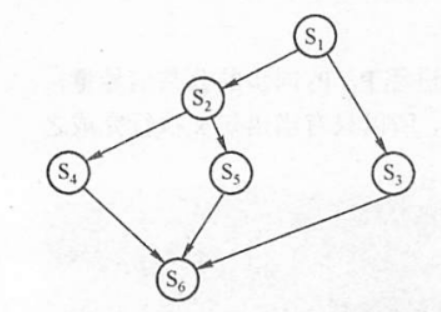
\includegraphics[width=0.4\textwidth]{image/chapter02/利用信号量实现前驱.png}
    \caption{利用信号量实现前驱关系}
\end{figure}

\begin{lstlisting}[language=C++]
semaphore s1_1 = s1_2 = s2_1 = s2_2 = s3 = s4 = s5 = 0;
S1() {        |  S2() {        |  S3() {
    ...       |      P(s1_1);  |      P(s1_2);
    V(s1_1);  |      ...       |      ...
    V(s1_2);  |      V(s2_1);  |      V(s3);
}             |      V(s2_2);  |  }
              |  }             |
----------------------------------------------
S4() {        |  S5() {        |  S6() {
    P(s2_1);  |      P(s2_2);  |      P(s4);
    ...       |      ...       |      P(s5);
    V(s4);    |      V(s_5);   |      P(s6);
}             |  }             |      ...
              |                |  }
\end{lstlisting}

    可以看见,其实依赖关系通过P(S)来阻塞,依赖关系一旦满足,则使用V(S)来解除依赖即可。因此,\emph{做题时,对于同步或多级同步来说,只需要V前P后即可满足。}

\subsection{管程}

    在信号量机制中,每个要访问临界资源的进程都必须自备同步PV操作。因此,一种新的进程同步工具————管程产生了,\emph{管程保证了进程互斥,且无需程序员自行实现互斥,降低了死锁的可能性。}

\subsubsection{管程的定义}

    \emph{系统中的各种硬件资源和软件资源,都可以用数据结构抽象地描述其资源,\color{red}即用少量信息和对资源所执行的操作来表征该资源,忽略内部结构和实现细节}。

    因此,如果用OOP的思想来看待,\emph{管程就是一个用户自描述的一个类,用共享数据结构抽象表示共享资源,然后通过类方法对共享资源进行操作。}

    \emph{管程(monitor),就是代表共享资源的数据结构,以及对该数据结构和实时操作的一组过程所组成的资源管理程序。}

    管程的基本特征为:

\begin{itemize}
    \item [1)] 局部于管程的数据只能被局部于管程的过程所访问
    \subitem 也就是说,管程中的共享数据,只允许通过管程中定义的方法操作
    \item [2)] 一个进程只有通过调用管城内的过程才能进入管程访问共享数据
    \subitem 和第一点所表达的意思是一致的
    \item [3)] \emph{\color{red}每次仅允许一个进程在管程中执行某个内部过程}
    \subitem 也就是说,管程是互斥的,管程中的操作,只能由一个进程访问,不允许多个进程同时执行。
\end{itemize}

\begin{figure}[!htbp]
    \centering
    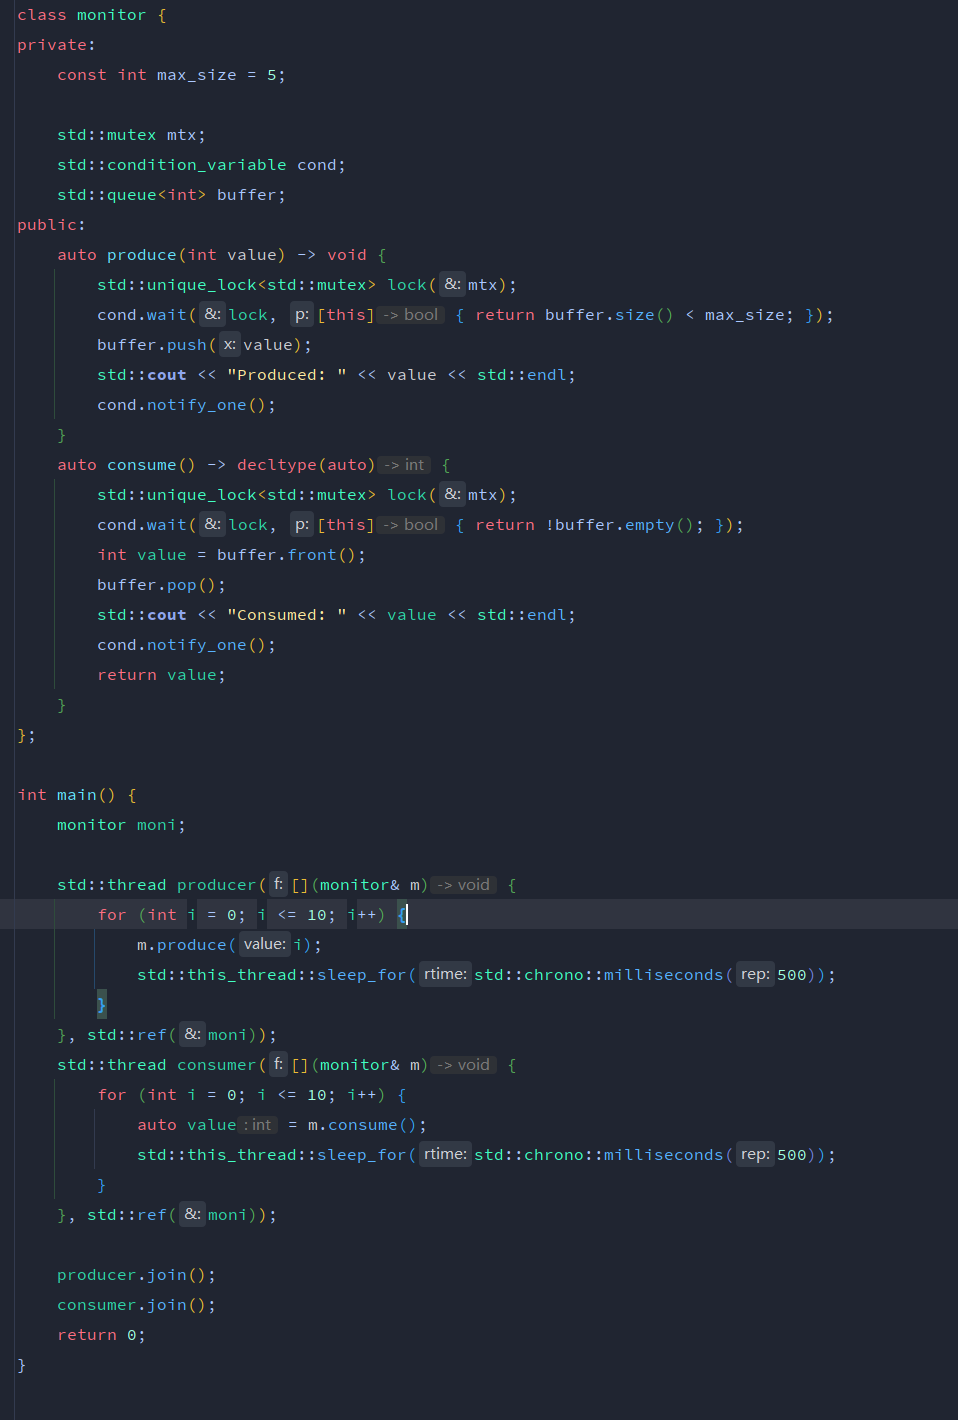
\includegraphics[width=0.8\textwidth]{image/chapter02/利用管程处理生产者消费者模型.png}
    \caption{利用管程处理生产者消费者模型}
\end{figure}

    如图2.12所示,在C++中利用互斥锁和条件变量自定义了一个管程(monitor)类,其中,buffer就是我们的缓冲区资源,而max\_size就是规定的最大数量。

    而produce和consume函数,就是对管程的操作过程,其中,里面的wait函数,用于条件变量的作用。